%% Author_tex.tex
%% V1.0
%% 2012/13/12
%% developed by Techset
%%
%% This file describes the coding for rsproca.cls

\documentclass[]{rsos}%%%%where rsos is the template name


\usepackage[T1]{fontenc}
\usepackage[utf8]{inputenc}


% tightlist command for lists without linebreak
\providecommand{\tightlist}{%
  \setlength{\itemsep}{0pt}\setlength{\parskip}{0pt}}

% From pandoc table feature
\usepackage{longtable,booktabs,array}
\usepackage{calc} % for calculating minipage widths
% Correct order of tables after \paragraph or \subparagraph
\usepackage{etoolbox}
\makeatletter
\patchcmd\longtable{\par}{\if@noskipsec\mbox{}\fi\par}{}{}
\makeatother
% Allow footnotes in longtable head/foot
\IfFileExists{footnotehyper.sty}{\usepackage{footnotehyper}}{\usepackage{footnote}}
\makesavenoteenv{longtable}


\usepackage{float}

%%%% *** Do not adjust lengths that control margins, column widths, etc. ***

%%%%%%%%%%% Defining Enunciations  %%%%%%%%%%%
\newtheorem{theorem}{\bf Theorem}[section]
\newtheorem{condition}{\bf Condition}[section]
\newtheorem{corollary}{\bf Corollary}[section]
%%%%%%%%%%%%%%%%%%%%%%%%%%%%%%%%%%%%%%%%%%%%%%%

\begin{document}


%%%% Article title to be placed here
\title{Supplementary Material - A systematic machine learning approach to assess biases in population data from mobile phone applications}

\author{
Carmen Cabrera$^{1}$,
Francisco Rowe$^{1}$}

\address{
  $^{1}$Geographic Data Science Lab, Department of Geography and Planning, University of Liverpool, Liverpool, United Kingdom.\\
  $^{}$}
%%%% Subject entries to be placed here %%%%
\subject{
Mobile phone data,
Human mobility,
Explainable AI,
Spatial analysis}

%%%% Keyword entries to be placed here %%%%
\keywords{
Mobile phone data,
Human mobility,
Digital trace data,
Population estimates,
Coverage bias,
Data representativeness,
Location,
Explainable AI,
Machine learning,
Spatial bias}

%%%% Insert corresponding author and its email address}
\corres{
  Carmen Cabrera, Francisco Rowe\\
  e-mail: \href{mailto:c.cabrera@liverpool.ac.uk}{\nolinkurl{c.cabrera@liverpool.ac.uk}}; \href{mailto:fcorowe@liverpool.ac.uk}{\nolinkurl{fcorowe@liverpool.ac.uk}}
}

%%%% Abstract text to be placed here %%%%%%%%%%%%
\begin{abstract}
Traditional sources of population data, such as censuses and surveys, are costly, infrequent, and often unavailable in crisis-affected regions. Mobile phone application data (MPD) offer near--real-time, high-resolution insights into population distribution, but their utility is undermined by unequal access to digital technologies, creating biases that threaten representativeness. Despite recognition of these issues, no standard framework exists to address such biases, limiting the reliability of MPD for research and policy. We develop and implement a systematic, replicable framework to quantify and explain population coverage bias in aggregated mobile phone application data without requiring individual-level attributes. The approach combines an indicator of population coverage bias with explainable machine learning to identify contextual drivers of spatial variation in bias. Using four datasets for the United Kingdom benchmarked against the 2021 census, we show that MPD achieve higher population coverage than national surveys, but biases persist across sources and subnational areas. Population coverage bias is strongly associated with demographic, socioeconomic, and geographic features, often in complex nonlinear ways. Contrary to common assumptions, multi-application datasets do not necessarily reduce bias compared to single-app sources. Our findings establish a foundation for bias assessment standards in MPD, offering practical tools for researchers, statistical agencies, and policymakers.
\end{abstract}
%%%%%%%%%%%%%%%%%%%%%%%%%%%

\providecommand{\EndFirstPage}{%
}

\maketitle

\newpage

\section{Alternative data aggregation approaches for Facebook data}\label{alternative-data-aggregation-approaches-for-facebook-data}

Facebook Population data was aggregated temporally by averaging daily
population counts over a month and then spatially, by aggregating it
into Local Authority Districts (LADs), ensuring alignment with official
census data. To test the robustness of the population coverage bias
indicator (Equation 3.2 in the main text) under data aggregation
strategies, we compared results from this chosen approach with
alternative ones. To this end, we examined the relationship between the
LAD-level bias indicator obtained from Facebook data according to the
chosen approach and from alternative aggregation approaches. We expect
to find strong linear correlations if the bias indicator is robust to
the aggregation approach. The robustness test is shown in Supplementary Figure \ref{fig:sensitivity}, where the x-axis shows the bias indicators under
the chosen method, while the y-axis shows alternative aggregation
approaches by: A) grouping into LADs, then averaging over a month; B)
averaging over a week from March 2021, then grouping into LADs; C)
grouping into LADs, then averaging over a week. For completeness we also
compare bias indicators derived from Facebook under the chosen
aggregation approach and bias indicators derived from other data
sources: D) Twitter/X, E) Multi-app 1, F) Mult-app 2.

Strong linear relationships are observed between Facebook bias
indicators across all aggregation approaches, with Pearson correlation
coefficients of 1, confirming robustness to aggregation choices. In
contrast, comparisons with other data sources show no such correlation,
indicating that different LADs exhibit larger biases depending on the
data source.

\begin{figure}[h]\label{fig:sensitivity}
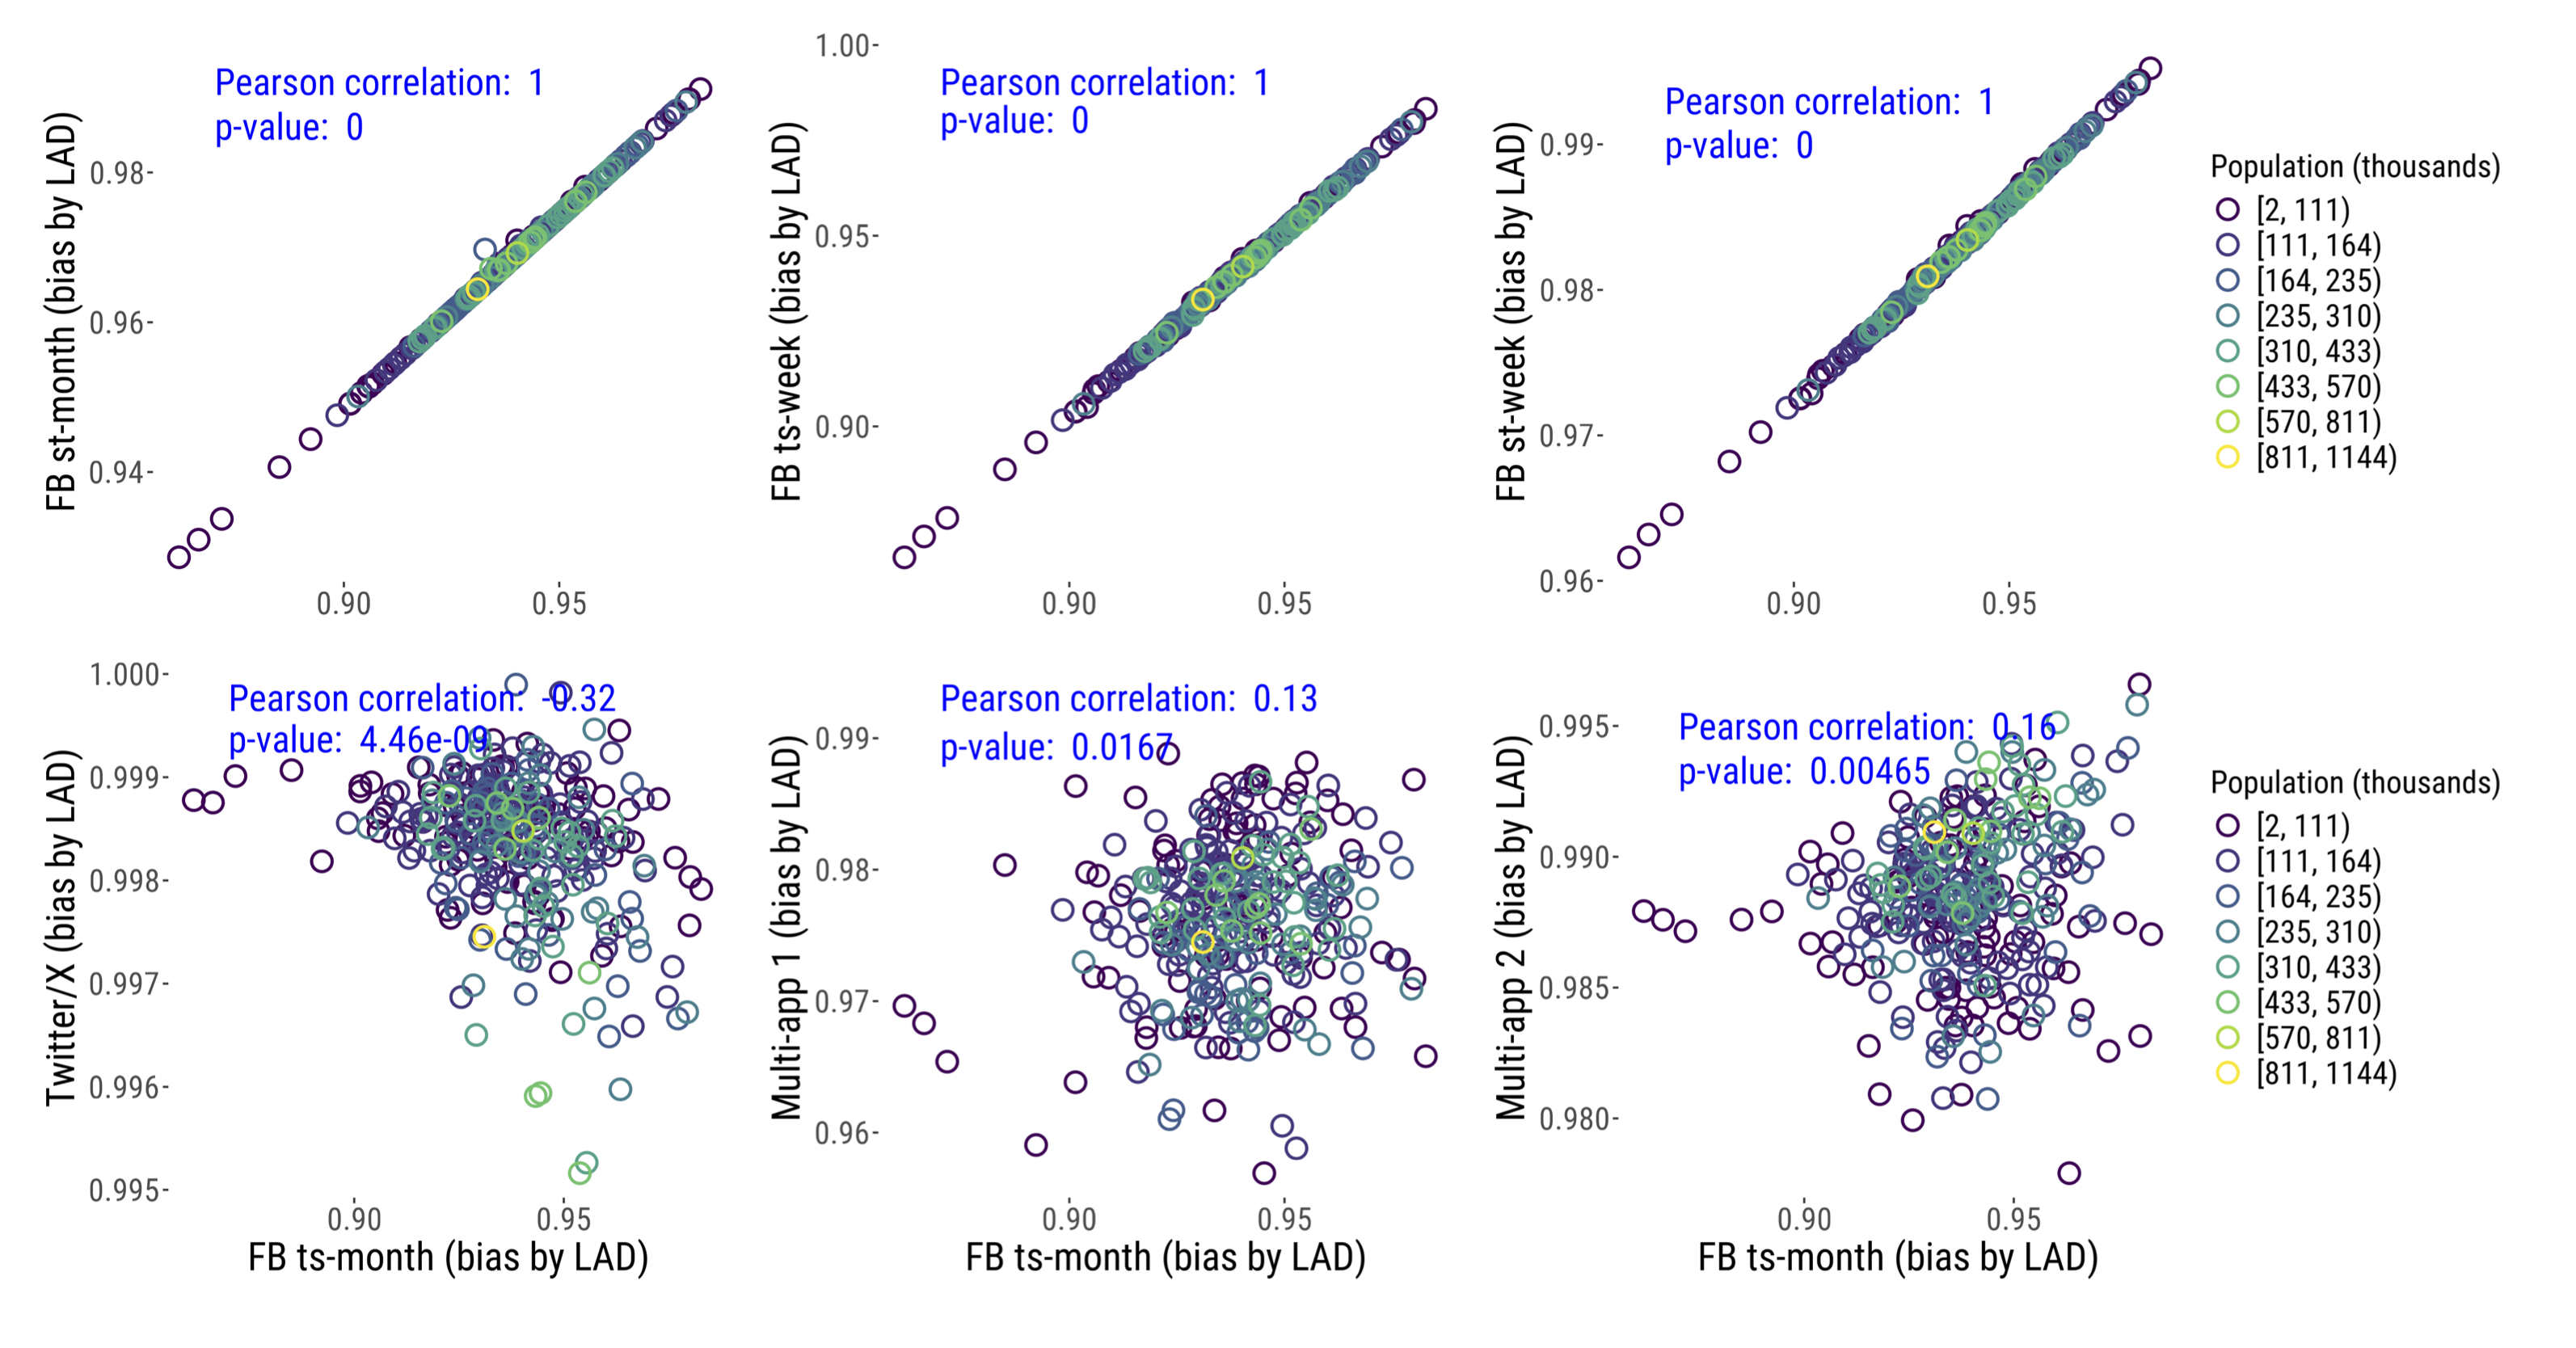
\includegraphics[width=\textwidth]{figures/Fig-compare-bias-size.png}
\caption{Robustness test of population coverage bias indicators derived from Facebook data, under alternative data aggregation approaches.}
\end{figure}

\newpage

\section{Testing for spatial autocorrelation in population coverage bias and covariates}\label{testing-for-spatial-autocorrelation-in-population-coverage-bias-and-covariates}

We analysed the spatial distribution of the population coverage bias
indicator across LADs. Figure 3 in the main text reports Moran's I
values computed using queen contiguity neighbourhoods. For comparison,
Supplementary Table \ref{fig:table-neighbour} presents Moran's I values and
associated p-values obtained under alternative spatial weighting
schemes.

\begin{table}[ht]\label{fig:table-neighbour}
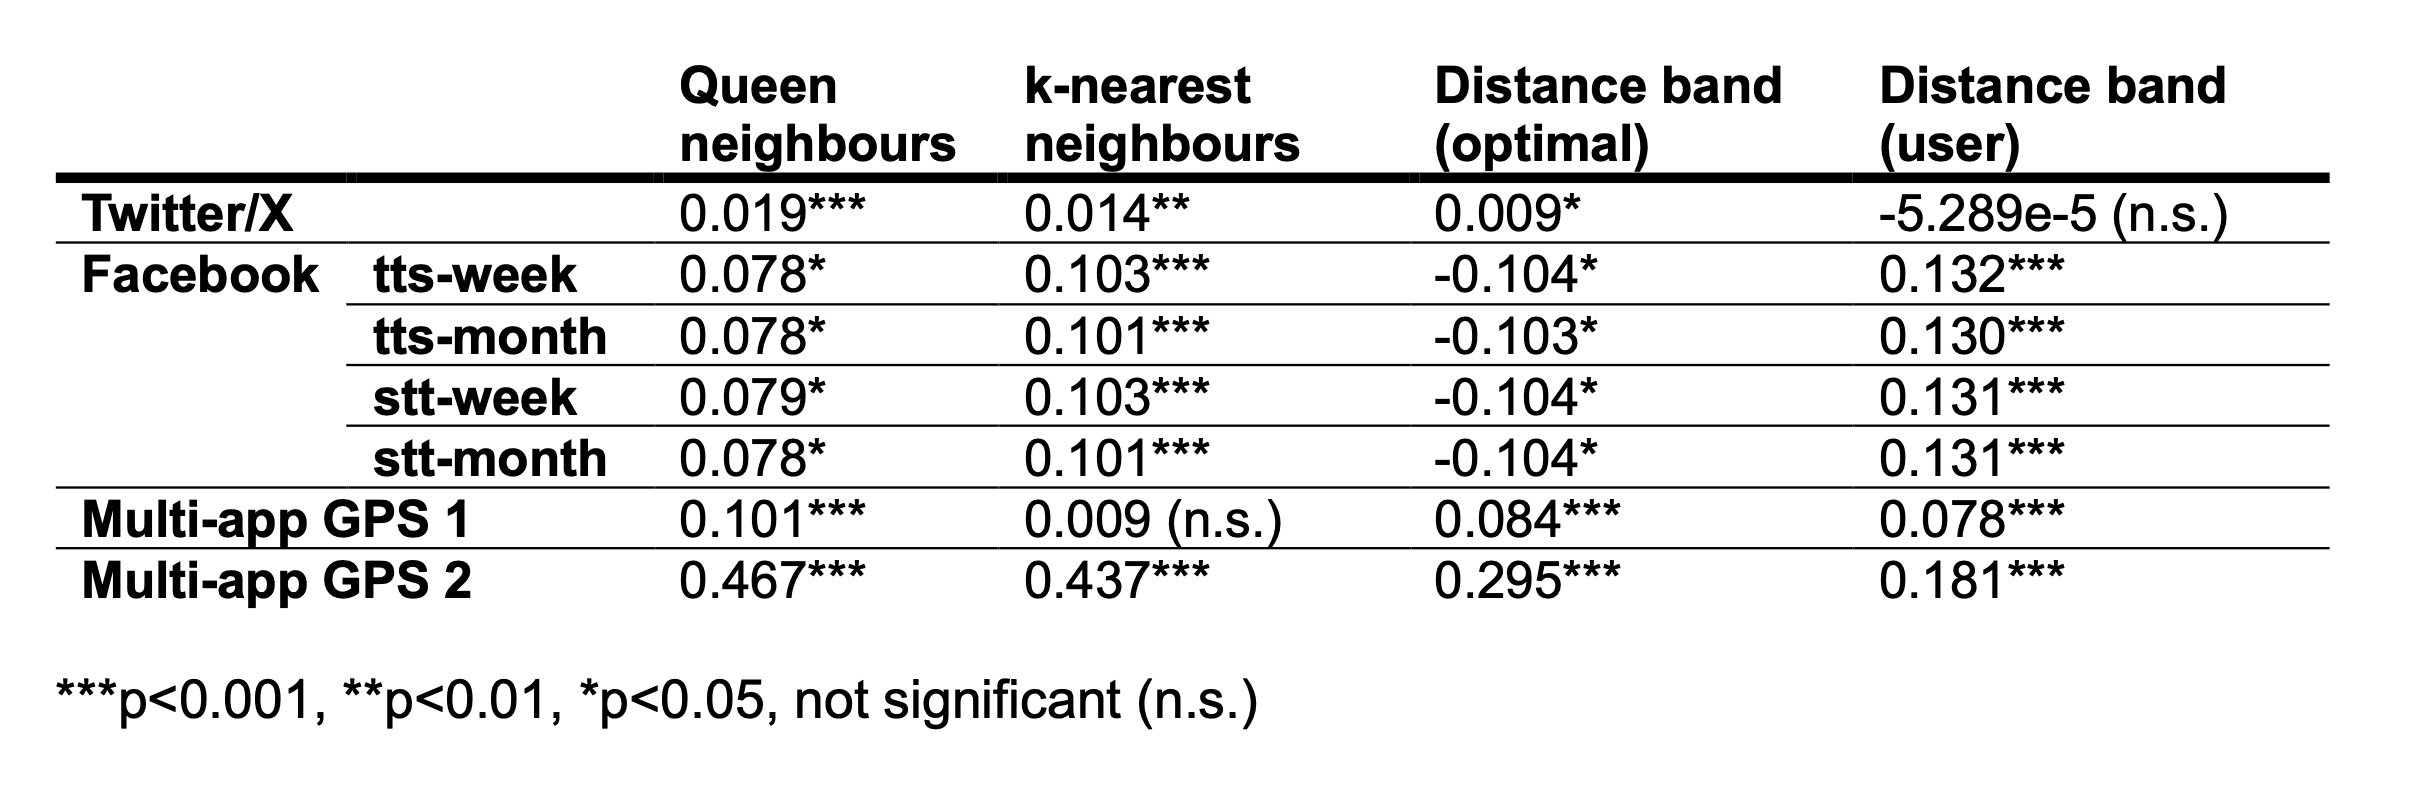
\includegraphics[width=\textwidth]{figures/Table-si.png}
\caption{Moran's I coefficients and significance,
computed according to four spatial weights schemes, 1) queen
neighbourhood, 2) k-nearest neighbours, 3) optimal distance band, and 4)
user-defined distance band.}
\end{table}

To complement the Moran's I assessment for the outcome variable, we also
computed Moran's I (queen contiguity) for each model covariate. This
provides a check of spatial autocorrelation in explanatory variables,
which is relevant when evaluating whether spatially blocked
cross-validation is warranted.

\begin{centering}
\begin{table}[ht]\label{fig:covariate-autocorrelation}
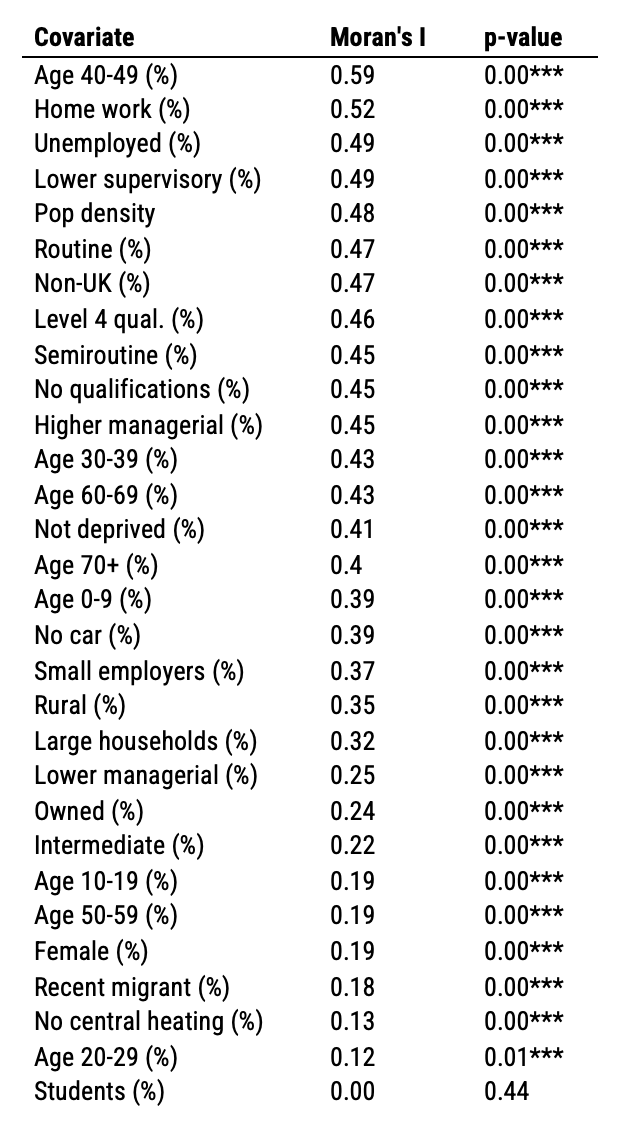
\includegraphics[width=0.5\textwidth]{figures/table-covariate-autocorrelation.png}
\caption{Spatial autocorrelation of model covariates measured using Moran's I under queen contiguity. The table reports Moran's I and associated p-values for each covariate, ordered by absolute Moran's I.}
\end{table}
\end{centering}

\newpage

\section{Residual assessments for proportional baseline}\label{residual-assessments-for-proportional-baseline}

This section reports supplementary tables for the proportional baseline
residual assessments described in the main text. Supplementary Table
\ref{fig:baseline-summary} summarises baseline fit and Moran's I of
residuals by data source. Supplementary Tables \ref{fig:corr-twitter} to
\ref{fig:corr-mapp2} report pairwise residual-covariate assessments for
each dataset, including Pearson, Spearman, and distance correlation, and
information criteria (AIC/BIC) for linear and GAM specifications.

\begin{table}[h]\label{fig:baseline-summary}
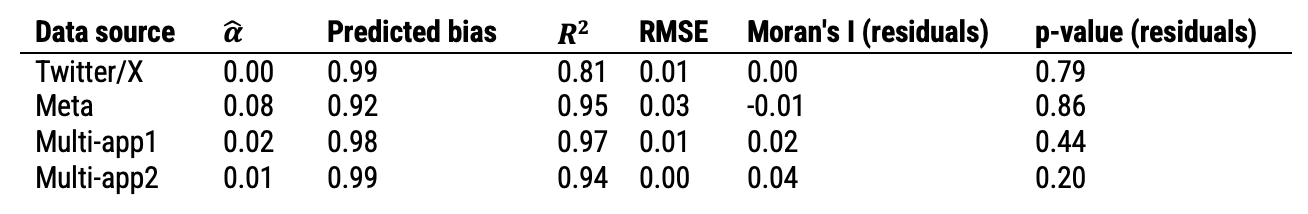
\includegraphics[width=0.95\textwidth]{figures/table-proportional-baseline-summary.png}
\caption{Baseline proportional model summary by data source, including estimated proportionality coefficient ($\hat{\alpha}$), model fit ($R^2$), and Moran’s I of residual bias.}
\end{table}

\begin{table}[h]\label{fig:corr-twitter}
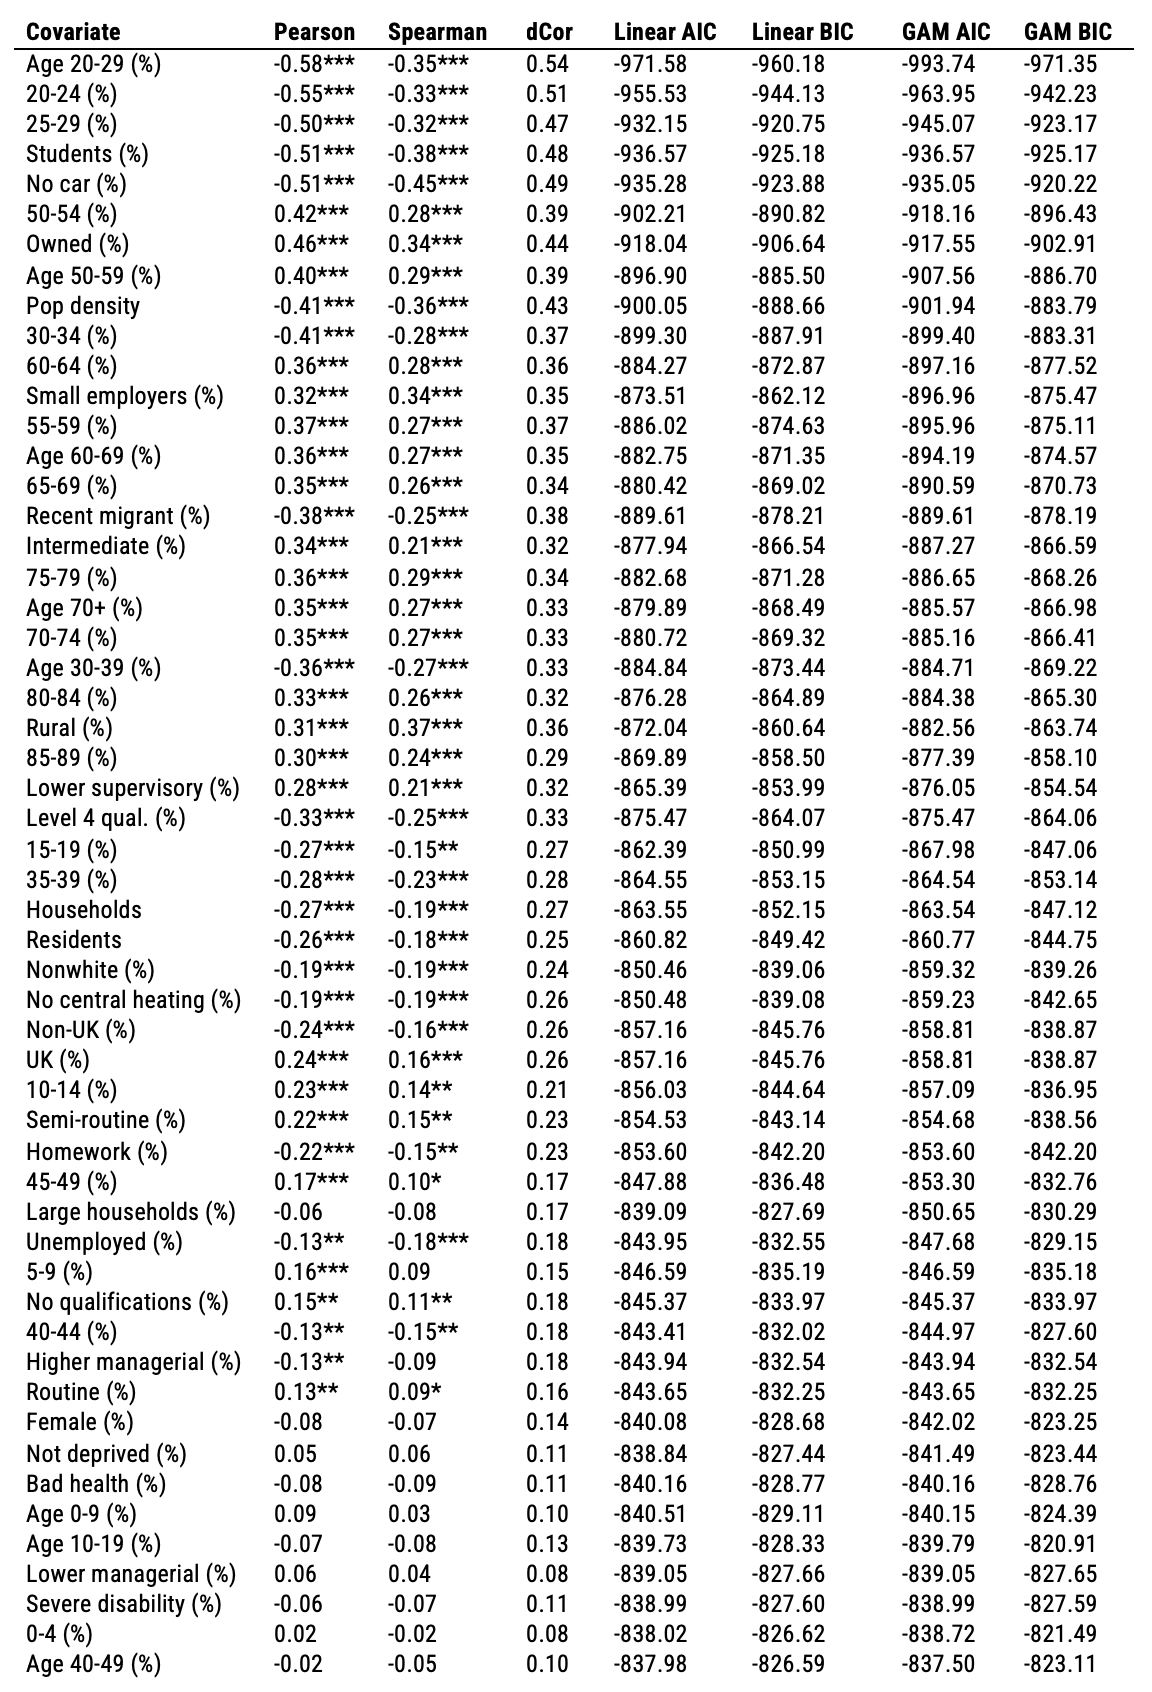
\includegraphics[width=0.95\textwidth]{figures/table-covariate-assessment-twitter.png}
\caption{Assessment of pairwise relationships between contextual covariates and residual for Twitter/X data. For each covariate, the table reports Pearson, Spearman and distance correlation with baseline residual bias, together with AIC and BIC for linear (OLS) and nonlinear (GAM, $k = 5$) models. Lower AIC/BIC indicates better fit.}
\end{table}

\begin{table}[h]\label{fig:corr-meta}
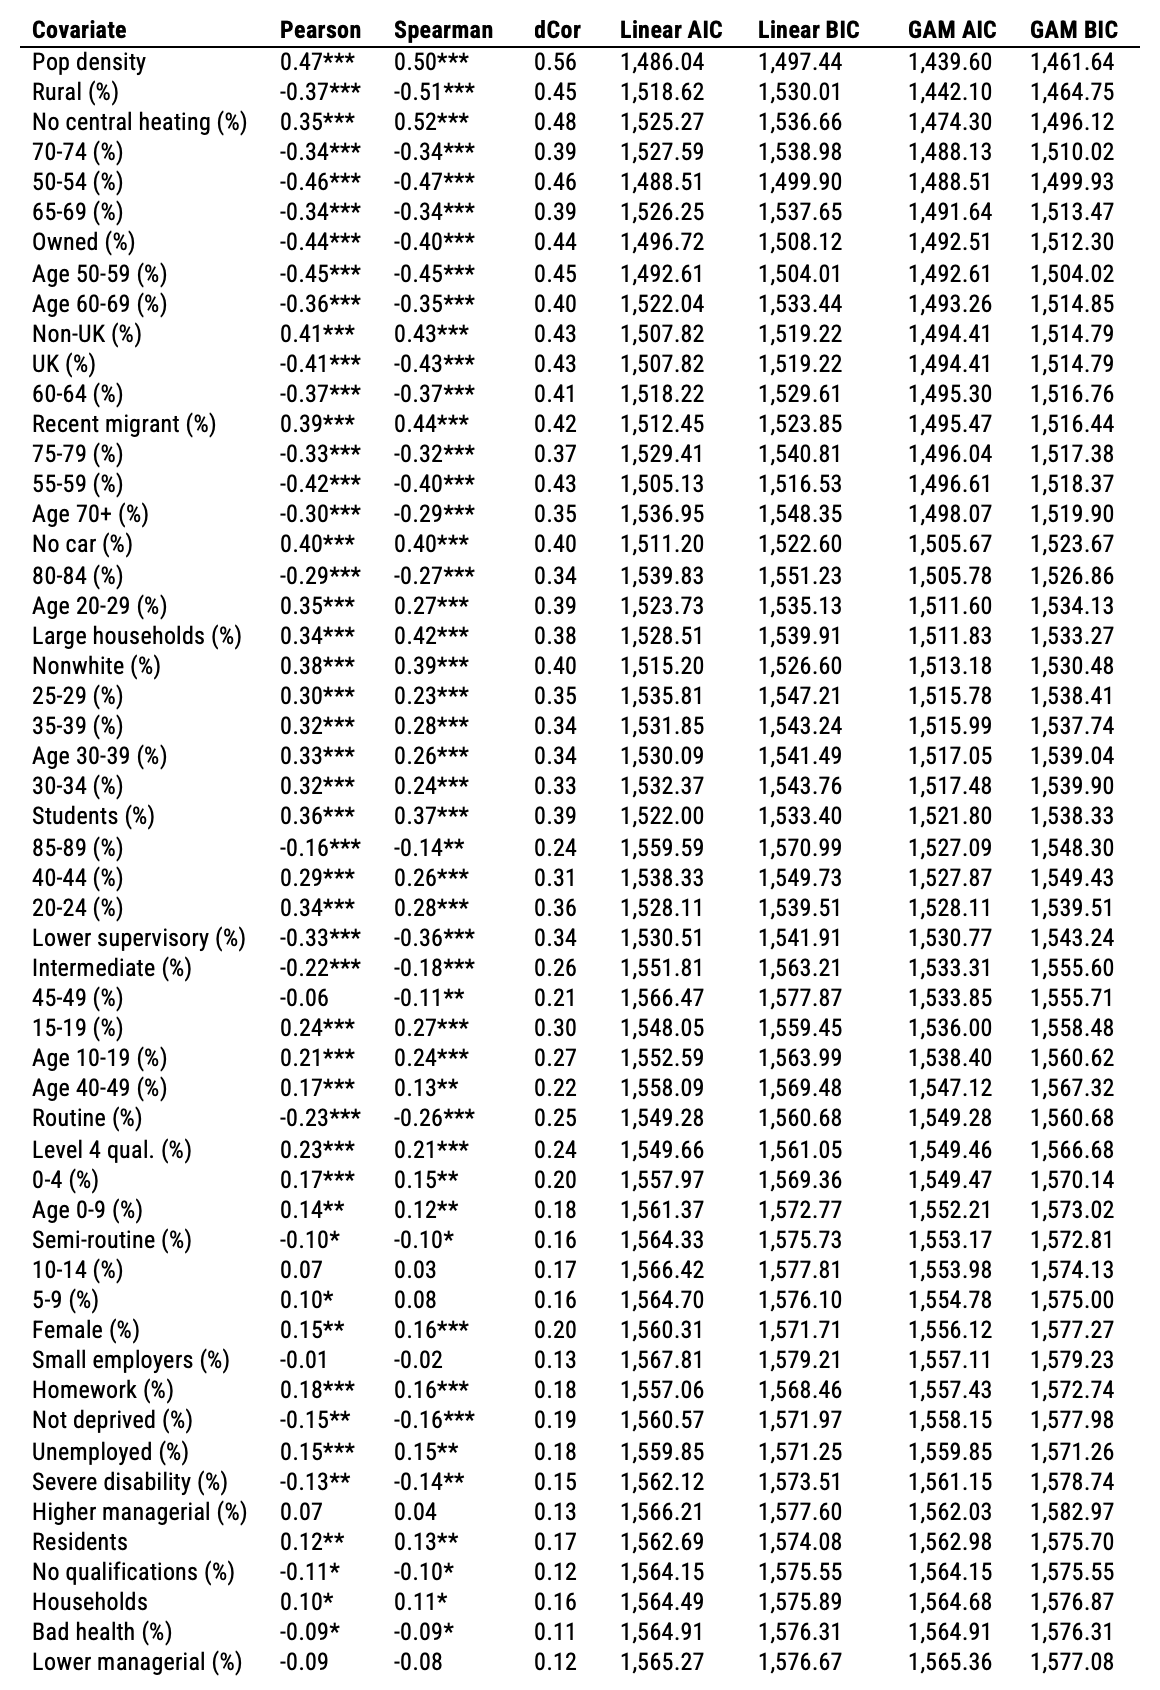
\includegraphics[width=0.95\textwidth]{figures/table-covariate-assessment-meta.png}
\caption{Assessment of pairwise relationships between contextual covariates and residual for Meta data. For each covariate, the table reports Pearson, Spearman and distance correlation with baseline residual bias, together with AIC and BIC for linear (OLS) and nonlinear (GAM, $k = 5$) models. Lower AIC/BIC indicates better fit.}
\end{table}

\begin{table}[h]\label{fig:corr-mapp1}
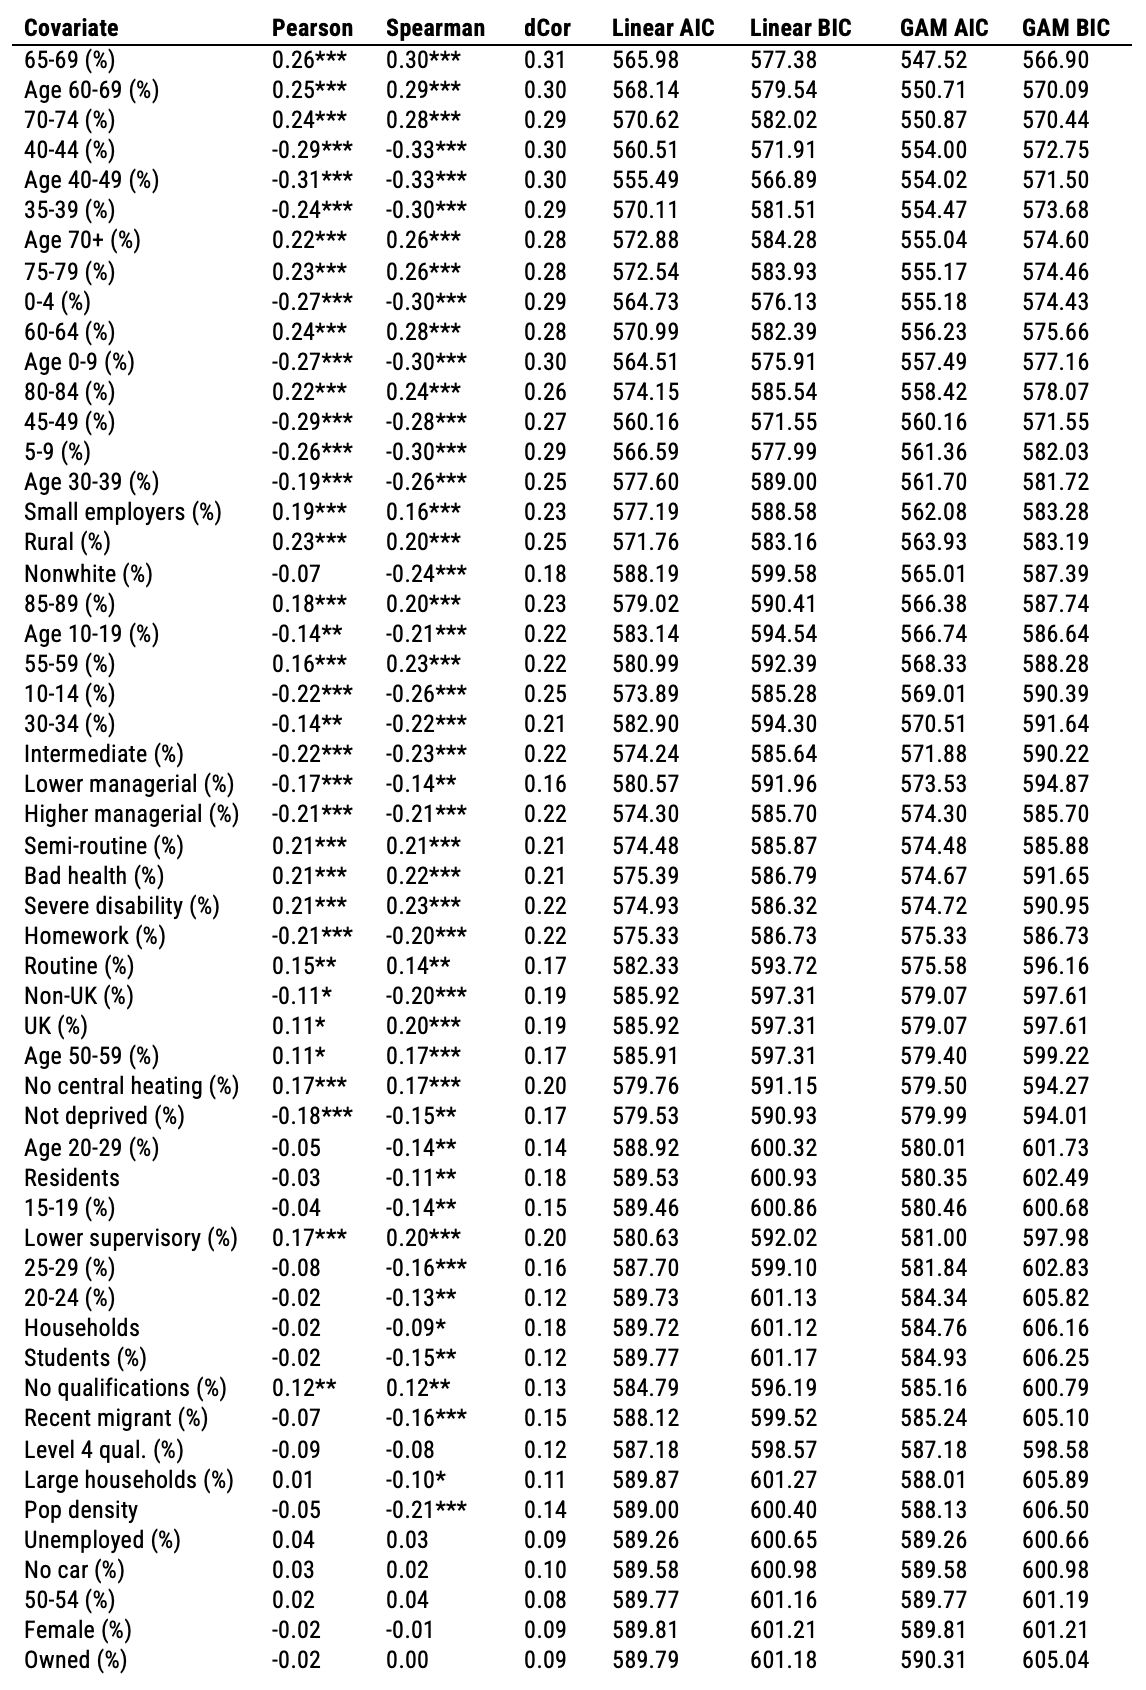
\includegraphics[width=0.95\textwidth]{figures/table-covariate-assessment-mapp1.png}
\caption{Assessment of pairwise relationships between contextual covariates and residual for Multi-app1 data. For each covariate, the table reports Pearson, Spearman and distance correlation with baseline residual bias, together with AIC and BIC for linear (OLS) and nonlinear (GAM, $k = 5$) models. Lower AIC/BIC indicates better fit.}
\end{table}

\begin{table}[h]\label{fig:corr-mapp2}
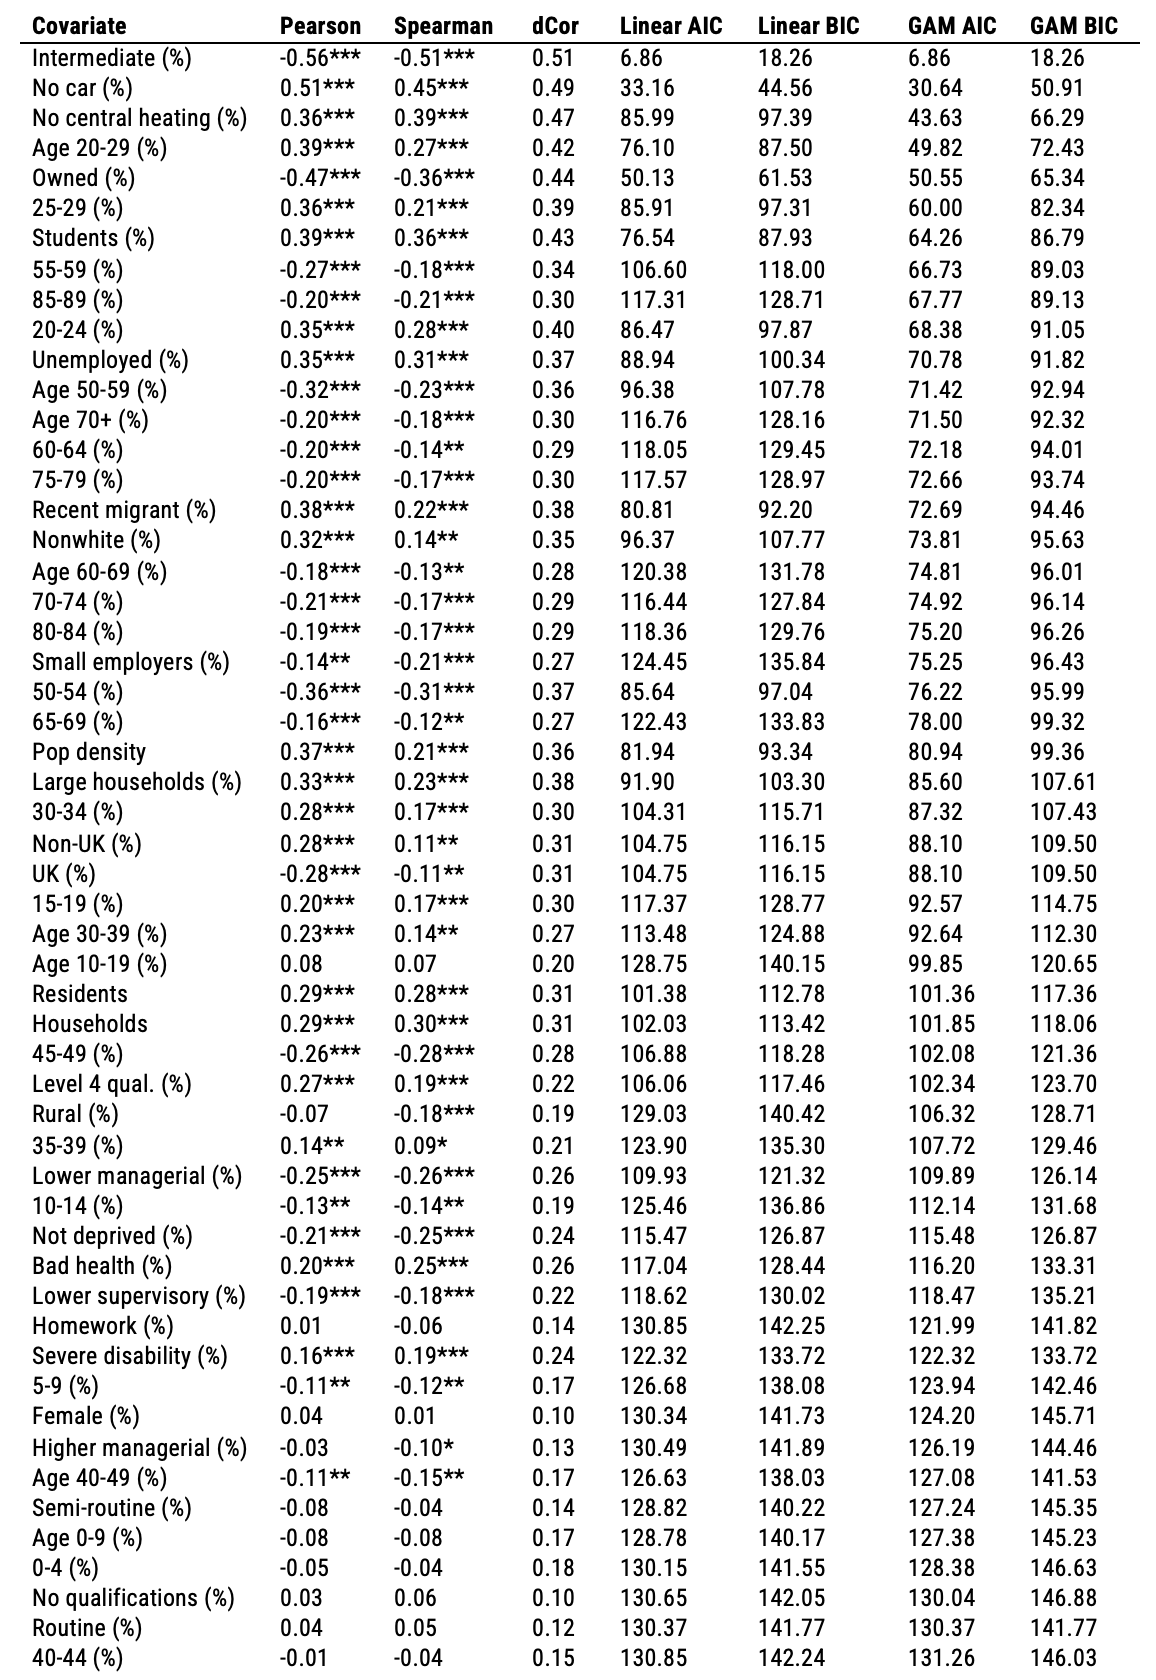
\includegraphics[width=0.95\textwidth]{figures/table-covariate-assessment-mapp2.png}
\caption{Assessment of pairwise relationships between contextual covariates and residual for Multi-app2 data. For each covariate, the table reports Pearson, Spearman and distance correlation with baseline residual bias, together with AIC and BIC for linear (OLS) and nonlinear (GAM, $k = 5$) models. Lower AIC/BIC indicates better fit.}
\end{table}

\section{Model performance}\label{model-performance}

\begin{table}[h]\label{fig:model-performance}
\centering
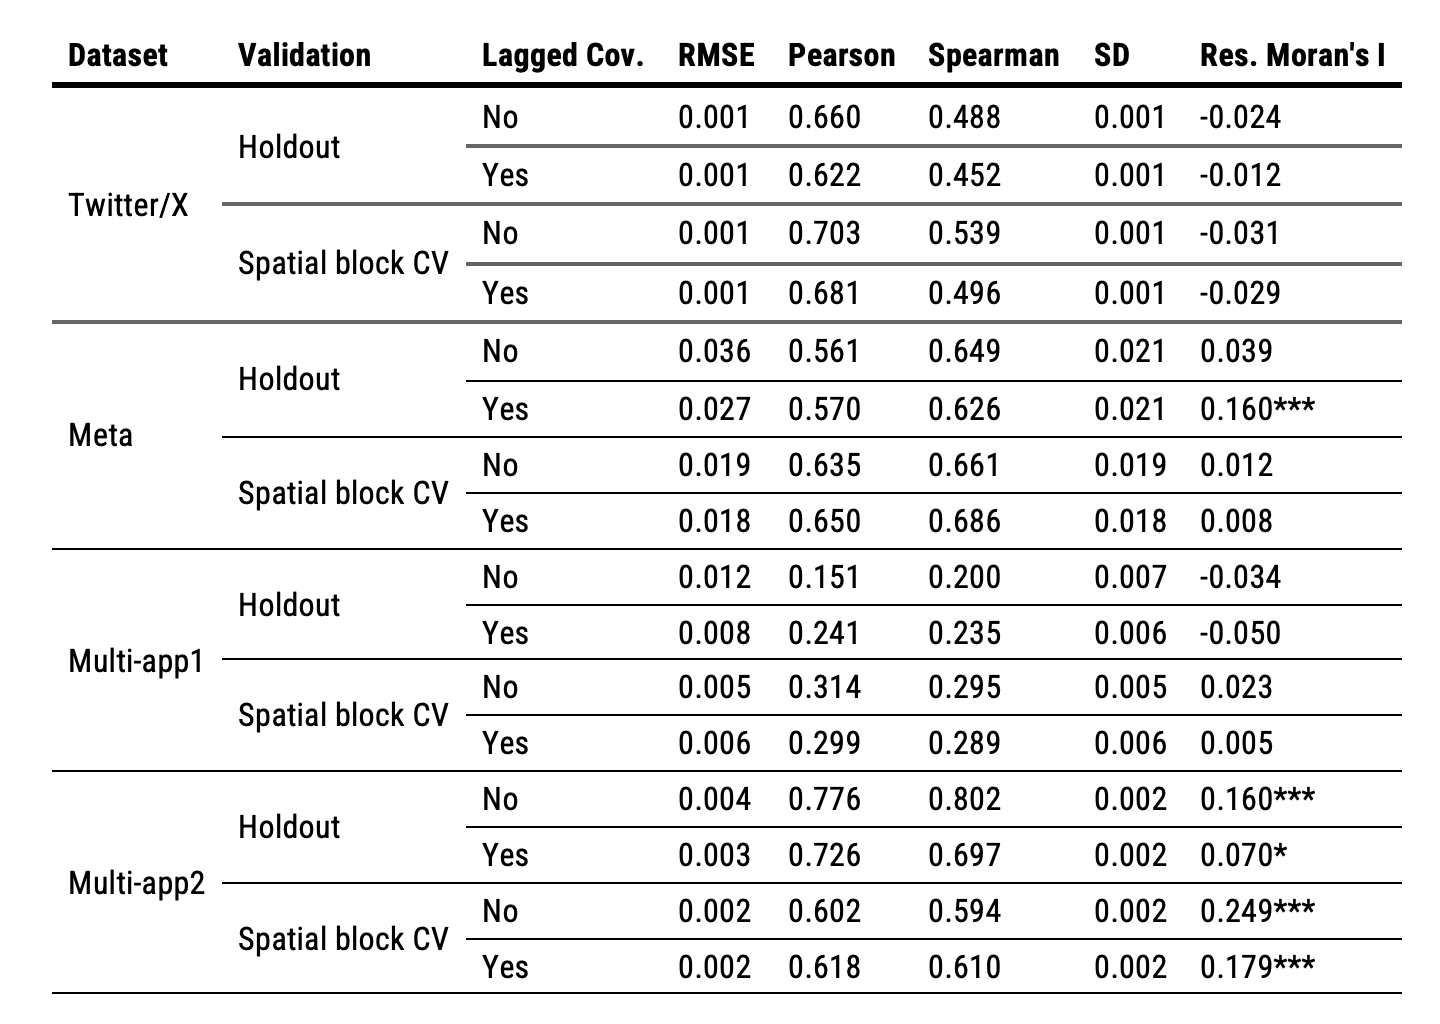
\includegraphics[width=0.9\textwidth]{figures/table-model-performance.png}
\caption{Comparison of machine-learning model performance across validation strategies and model specifications. For each dataset, the table reports out-of-sample performance for random holdout and spatial block cross-validation models, estimated with and without spatially lagged covariates. Performance is evaluated using the root mean squared error (RMSE), Pearson correlation, Spearman correlation, standard deviation of prediction error and Moran's $I$ of model residuals.}
\end{table}

\begin{figure}[h]\label{fig:variable-importance}
\centering
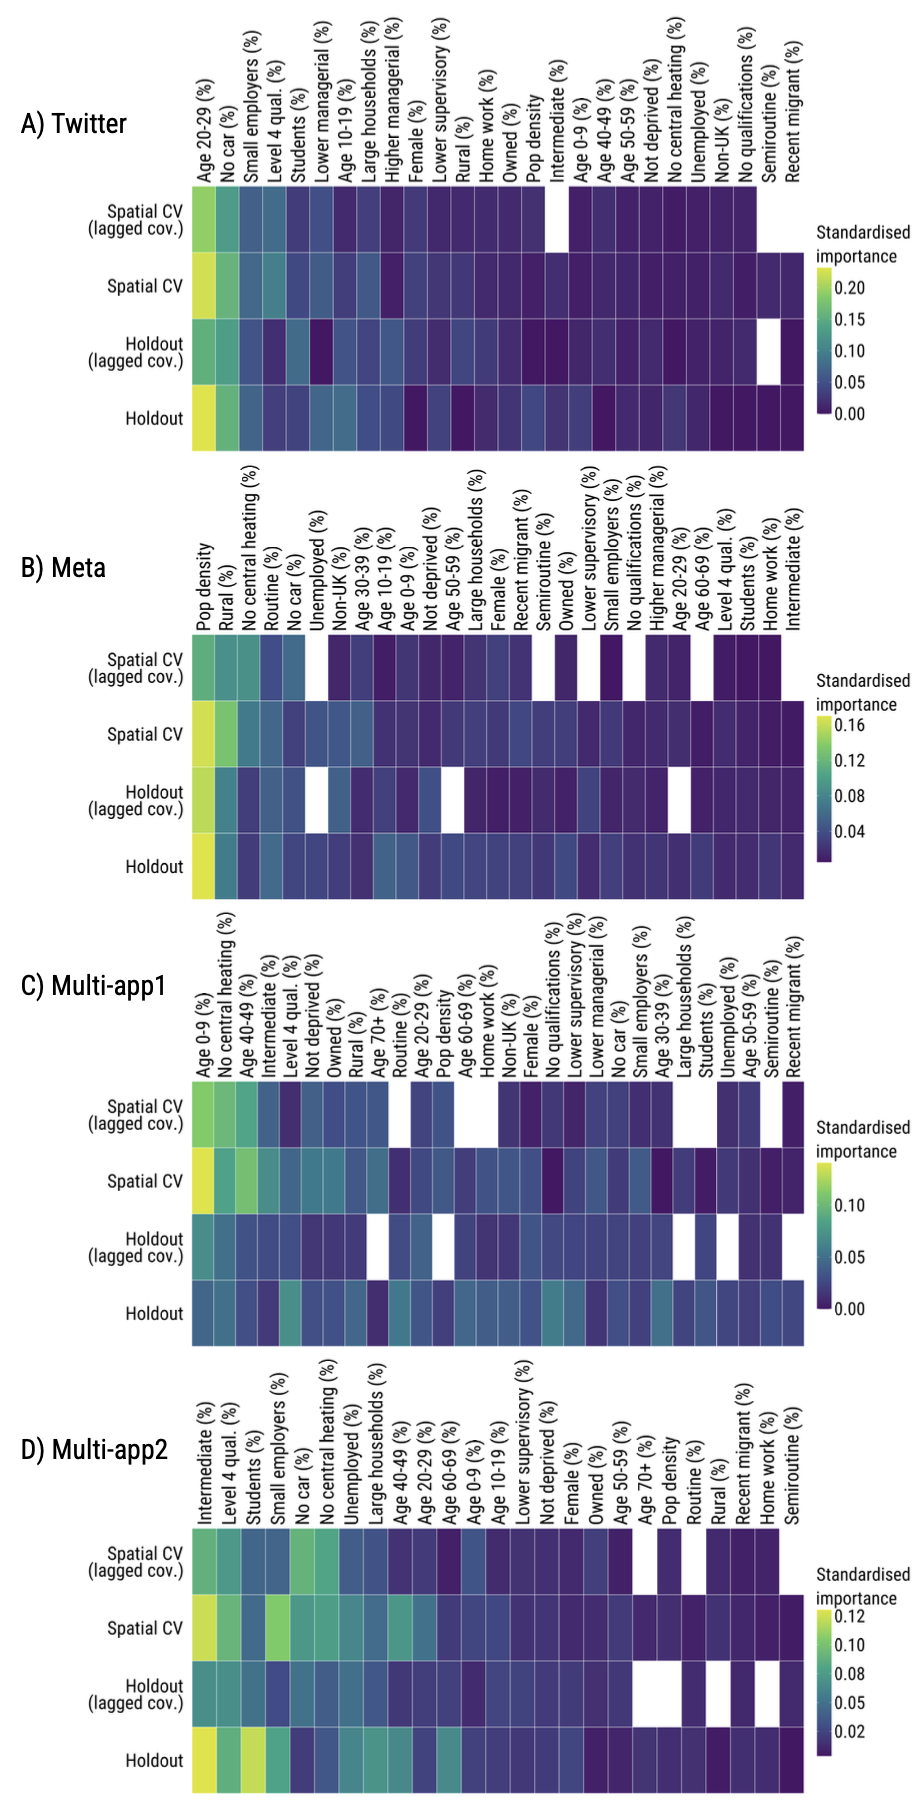
\includegraphics[width=0.8\textwidth]{figures/variable-importance.png}
\caption{Robustness test of variable importance across model validation strategies. Each panel reports standardised feature importance scores from models estimated under random holdout and spatial block cross-validation, with and without spatially lagged covariates. For readability, only the original non-lagged contextual covariates are displayed, including in specifications that also contain lagged covariates. The similarity of the importance profiles indicates that the main contextual drivers of population coverage bias are stable across validation strategies.}
\end{figure}

\begin{table}[h]\label{fig:model-performance}
\centering
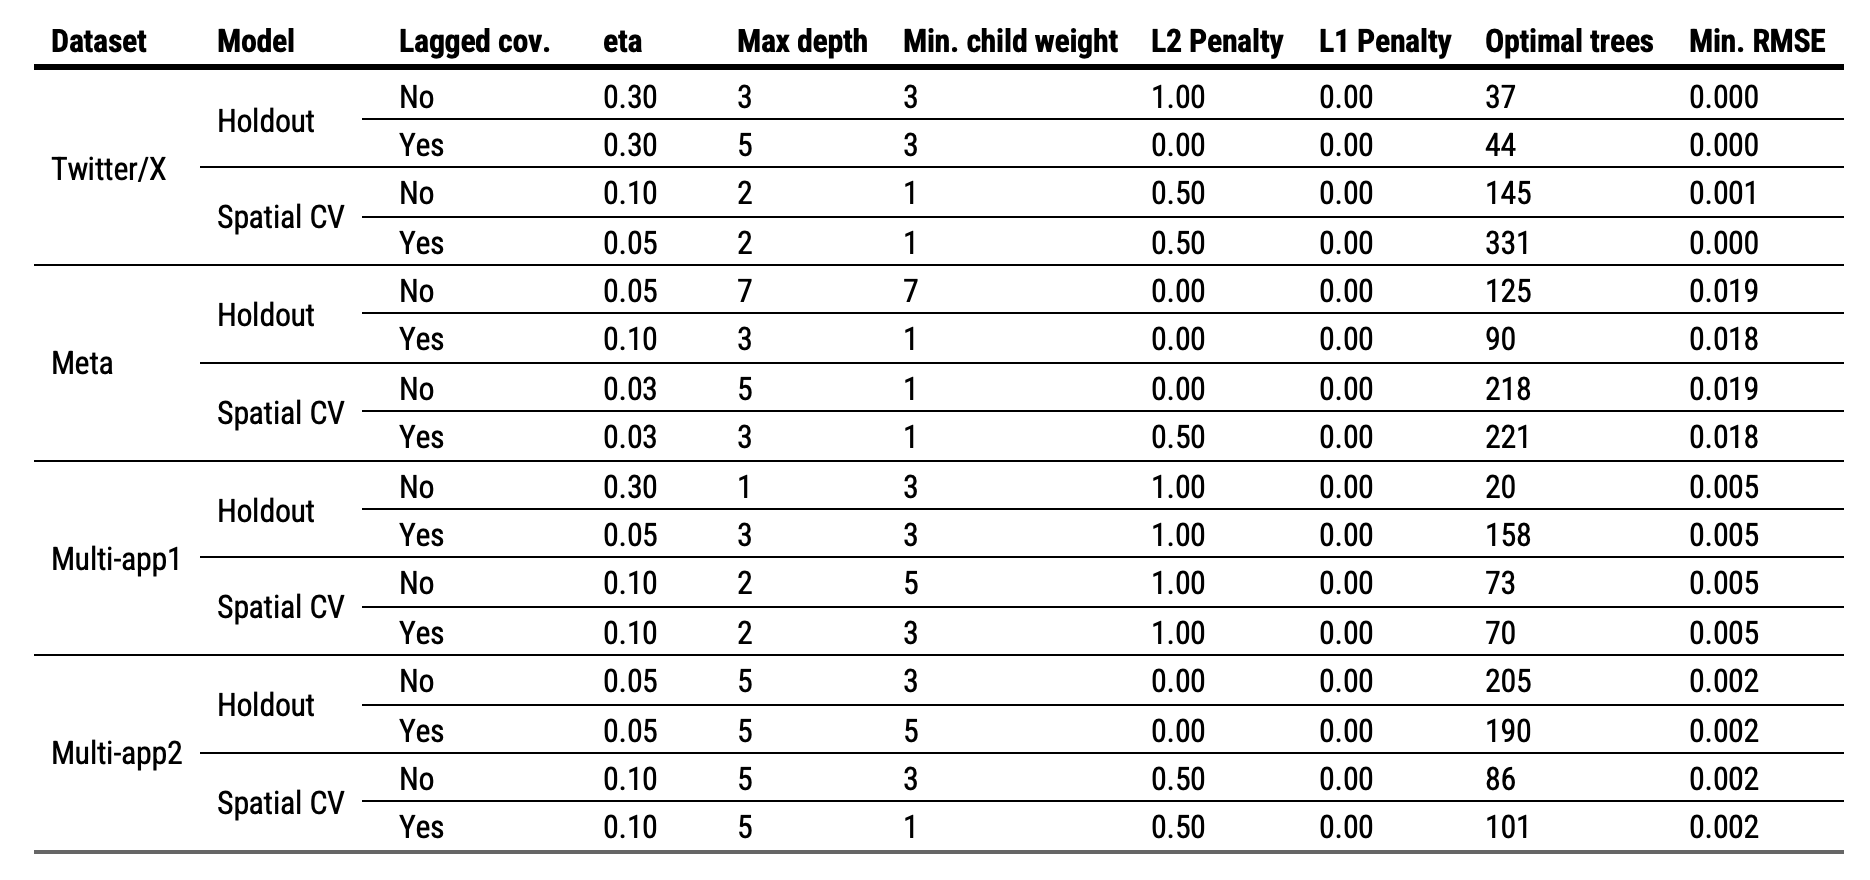
\includegraphics[width=\textwidth]{figures/table-hyperparameters.png}
\caption{Selected XGBoost hyperparameters across datasets and model specifications. For each dataset, the table reports the tuned hyperparameters for random holdout and spatial block cross-validation models, estimated with and without spatially lagged covariates. Parameters include learning rate (\textit{eta}), maximum tree depth, minimum child weight, row and column subsampling ratios, L1 and L2 regularisation penalties, the selected number of trees and the minimum out-of-sample RMSE.}
\end{table}

\begin{figure}[h]\label{fig:xgb-residual-maps}
\centering

\includegraphics[width=0.9\textwidth]{figures/xgb-residual-maps.png}
\caption{Model residuals across local authority district areas based on our main XGBoost model reported in the manuscript}
\end{figure}

\ethics{This research was conducted in accordance with the ethical standards of the University of Liverpool. All data used were anonymised and analysed at an aggregate level. No identifiable personal data were accessed or processed by the authors.}

\dataccess{Please see data accessibility in the Data section. Code is openly available at \url{https://github.com/de-bias/bias-detection}.}

\aucontribute{Both authors contributed equally.}

\competing{The authors declare that they have no conflicts of interest relevant to this work.}

\funding{This work was supported by the Economic and Social Research Council (ESRC) through Smart Data Research UK programme {[}Project reference: ES/Y010787/1{]}.}

\disclaimer{Please provide disclaimer text here.}

\ack{The authors acknowledge the support of UK ESRC and of project partners: the International Organization for Migration (IOM), Meta Platforms, Inc., and Prof.~Esteban Moro.}

\bibliographystyle{RS}
\bibliography{sample.bib}


\end{document}
